
%%%%%%%%%%%%%%%%%%%%%%%%%%%%%%%%%%%%%%%%%%%%%%%%%%%%%%%%%%%%%%%%%%%%%%%%%%%%%%%%%%%%%%%
%%%%%%%%%%%%%%%%%%%%%%%%%%%%%%%%%%%%%%%%%%%%%%%%%%%%%%%%%%%%%%%%%%%%%%%%%%%%%%%%%%%%%%%
%%%%%%%%%%%%%%%%%%%%%%%%%%%%%%%%%%%%%%%%%%%%%%%%%%%%%%%%%%%%%%%%%%%%%%%%%%%%%%%%%%%%%%%
\section{Serie de Taylor de $d(x)$, $e(\VECTOR{x})$ e $\VECTOR{f}(\VECTOR{x})$}
\label{def:taylor}


\index{Serie de Taylor!$d:\mathbb{R} \rightarrow \mathbb{R}$}
\begin{proposition}[Serie de Taylor de $d(x)$:]\label{prop:taylord}
Dada uma função $d:\mathbb{R}\rightarrow \mathbb{R}$ com variável $x \in \mathbb{R}$;
infinitamente diferenciável em $a \in \mathbb{R}$;
esta pode ser expressada mediante uma somatória, em serie de Taylor 
\cite[pp. 764]{stewart2008calculus} \cite[pp. 281]{telles2015matematica} \cite{Taylor} 
ao redor de $a$, como
mostra a Eq. (\ref{eq:taylord1}),% onde $\left.\frac{\partial^k d(x)}{\partial x^k}\right|_{x=a}\equiv d^{(k)}(a) $.
\begin{equation}\label{eq:taylord0a}
\left.\frac{\partial^k d(x)}{\partial x^k}\right|_{x=a}\equiv d^{(k)}(a) 
\end{equation}
\begin{equation}\label{eq:taylord1}
  d(x)=d(a)
      ~+\frac{d'(a)}{1!} (x-a)
      ~+\frac{d''(a)}{2!} (x-a)^{2}
      ~+\cdots 
      ~+\frac{d^{(k)}(a)}{k!} (x-a)^{k}
      ~+\cdots 
\end{equation}
A equação pode ser escrita de forma mais compacta mediante uma somatória  como mostra a Eq. (\ref{eq:taylord2}),
\begin{equation}\label{eq:taylord2}
  d(x)=\sum\limits_{k=0}^{+\infty} \frac{d^{(k)}(a)}{k!} (x-a)^{k}.
\end{equation}
\end{proposition}


\begin{example}[Serie de Taylor do $cos(x)$:]
Podem ser vistas aproximações da função $d(x)=cos(x)$, 
mediante o uso da Proposição \ref{prop:taylord} onde é descrita a serie de Taylor ao redor do ponto $a=0$;
aqui é truncada a serie ate a derivada de ordem $4$, $8$ e $10$,
obtendo as aproximações $d_4(x)$, $d_8(x)$ e $d_{10}(x)$,
como pode ser visto na Fig. \ref{fig:taylore}.
\begin{equation}
d^{(k)}(x)=
\left\{
\begin{matrix}
cos(x) & ~if & (k~mod~4)=0\\
-sin(x)& ~if & (k~mod~4)=1\\
-cos(x)& ~if & (k~mod~4)=2\\
sin(x) & ~if & (k~mod~4)=3
\end{matrix}
\right.
\quad \rightarrow \quad
d^{(k)}(0)=
\left\{
\begin{matrix}
1 & ~if & (k~mod~4)=0\\
0& ~if & (k~mod~4)=1\\
-1& ~if & (k~mod~4)=2\\
0 & ~if & (k~mod~4)=3
\end{matrix}
\right.
\end{equation}

\begin{equation}
d_{4}(x)=
1
-\frac{x^{2}}{2!} 
+\frac{x^{4}}{4!},
\qquad 
d_{8}(x)=
1
-\frac{x^{2}}{2!} 
+\frac{x^{4}}{4!} 
-\frac{x^{6}}{6!} 
+\frac{x^{8}}{8!}, 
\end{equation}
\begin{equation}
d_{10}(x)=
1
-\frac{x^{2}}{2!} 
+\frac{x^{4}}{4!} 
-\frac{x^{6}}{6!} 
+\frac{x^{8}}{8!} 
-\frac{x^{10}}{10!} 
\end{equation}
\end{example}

\begin{figure}[!h]
  \centering
    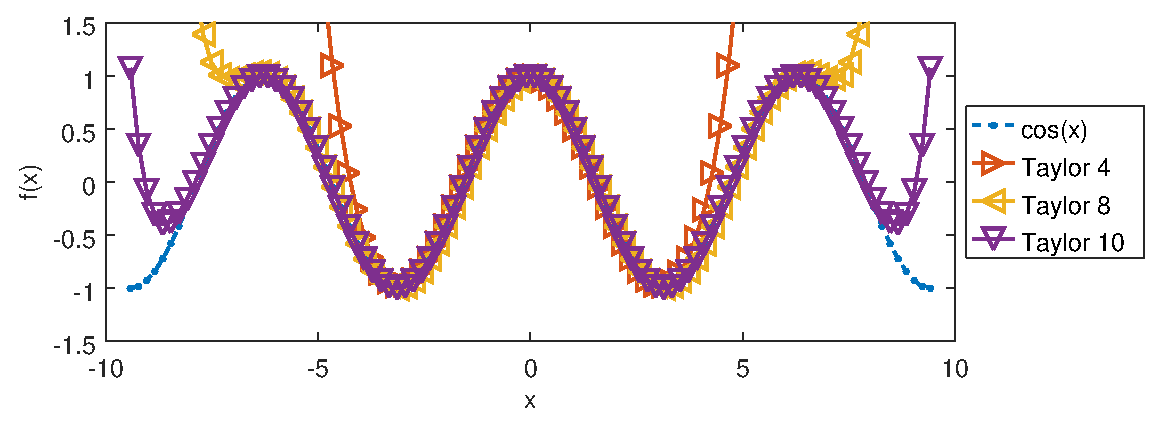
\includegraphics[width=0.90\textwidth]{chapters/funcoes/mcode/taylore.eps}
  \caption{Aproximação da função $cos(x)$ usando a serie de Taylor truncada.}
    \label{fig:taylore}
\end{figure}
 
%%%%%%%%%%%%%%%%%%%%%%%%%%%%%%%%%%%%%%%%%%%%%%%%%%%%%%%%%%%%%%%%%%%%%%%%%%%%%%%%%%%%%%%
 \index{Serie de Taylor!$f:\mathbb{R}^{N}\rightarrow \mathbb{R}$}
\begin{proposition}[Serie de Taylor de $f(\VECTOR{x})$]\label{prop:taylore}
Dada uma função $f:\mathbb{R}^{N}\rightarrow \mathbb{R}$ com variável $\VECTOR{x} \in \mathbb{R}^{N}$, vetor coluna;
infinitamente diferenciável em $\VECTOR{a} \in \mathbb{R}^{N}$;
esta pode ser expressada mediante uma somatória, em serie de Taylor 
\cite[pp. 187, 207]{zhang2017matrix} \cite{Taylor}  ao redor de $\VECTOR{a}$, como
mostra a Eq. (\ref{eq:taylore1}),
\begin{equation}\label{eq:taylore1}
f(\VECTOR{x}) =\sum _{k_{1}=0}^{\infty }\cdots \sum _{k_{N}=0}^{\infty }\left.\left({\frac {\partial ^{k_{1}+\cdots +k_{N}}f(\VECTOR{x})}{\partial x_{1}^{k_{1}}\cdots \partial x_{N}^{k_{N}}}}\right)\right|_{\VECTOR{x}=\VECTOR{a}} {\frac {(x_{1}-a_{1})^{k_{1}}\cdots (x_{N}-a_{N})^{k_{N}}}{k_{1}!\cdots k_{N}!}}
\end{equation}

Outra forma alternativa de expressar a função anterior é usando vetores e matrizes,
como na Eq. (\ref{eq:taylore2}).
\begin{equation}\label{eq:taylore2}
  f(\VECTOR{x})=f(\VECTOR{a})
      ~+ \triangledown f(\VECTOR{a})^{\transpose} (\VECTOR{x}-\VECTOR{a})
      ~+\frac{1}{2!}(\VECTOR{x}-\VECTOR{a})^{\transpose} \MATRIX{H(\VECTOR{a})}  (\VECTOR{x}-\VECTOR{a})
      ~+\cdots 
\end{equation}
Onde o vector $\triangledown f(\VECTOR{x})\equiv \frac{\partial f(\VECTOR{x})}{\partial \VECTOR{x} }$ 
(também chamado \hyperref[def:gradient]{gradiente}),
e a matriz $\MATRIX{H}(\VECTOR{x})\equiv \frac{\partial }{\partial \VECTOR{x}} \left( \frac{\partial f(\VECTOR{x})}{ \partial \VECTOR{x}^{\transpose} }\right)$
(também chamada matriz \hyperref[def:hessian]{Hessiana}).
\end{proposition}

%%%%%%%%%%%%%%%%%%%%%%%%%%%%%%%%%%%%%%%%%%%%%%%%%%%%%%%%%%%%%%%%%%%%%%%%%%%%%%%%%%%%%%%
\index{Serie de Taylor!$\VECTOR{f}:\mathbb{R}^{N}\rightarrow \mathbb{R}^{M}$}
\begin{proposition}[Serie de Taylor de $\VECTOR{f}(\VECTOR{x})$]\label{prop:taylorf}
Dada uma função de contra-domino vectorial $\VECTOR{f}:\mathbb{R}^{N}\rightarrow \mathbb{R}^{M}$, 
sendo $\VECTOR{f}$ um vector coluna, com variável $\VECTOR{x} \in \mathbb{R}^{N}$, vetor coluna;
infinitamente diferenciável em $\VECTOR{a} \in \mathbb{R}^{N}$;
esta pode ser expressada mediante uma somatória, em serie de Taylor 
\cite[pp. 393]{levine1999control} \cite{Taylor} ao redor de $\VECTOR{a}$, como
mostra a Eq. (\ref{eq:taylorf1}),
\begin{equation}\label{eq:taylorf1}
\VECTOR{f}(\VECTOR{x}) =\VECTOR{f}(\VECTOR{a})
      ~+ \MATRIX{J}(\VECTOR{a}) (\VECTOR{x}-\VECTOR{a})
      ~+\cdots 
\end{equation}

Onde a matriz $\MATRIX{J}(\VECTOR{x})\equiv \frac{\partial \VECTOR{f}(\VECTOR{x})}{\partial \VECTOR{x}^{\transpose} }$,
também conhecido como matriz \hyperref[def:jacobian]{Jacobiana} de $\VECTOR{f}(\VECTOR{x})$.
\end{proposition}
